\documentclass[10pt,reqno]{book}
\usepackage{amsmath,amssymb,amsfonts,amsthm}
\usepackage{graphics,tikz,caption}
\usepackage{emptypage}
\usepackage{pgfplots} 
\usepackage{listings}
\usepackage{booktabs}
\usepackage{graphicx}
\usepackage{ mathrsfs }
\usepackage{bm}
\usepackage{tikz-3dplot}
\usepackage{bigints}
\usepackage{pbox}
\usepackage{venndiagram}
\usepackage{enumitem}
\usetikzlibrary{patterns}
\usetikzlibrary{3d}
\graphicspath{ {images/} }
\usetikzlibrary{arrows,positioning,shapes,fit,calc}
\pgfplotsset{compat=1.8}

\renewcommand{\theenumi}{\Alph{enumi}}


\DeclareGraphicsExtensions{.pdf}
\parindent 1cm
\parskip 0.2cm
\topmargin 0.2cm
\oddsidemargin 1cm
\evensidemargin 0.5cm
\textwidth 15cm
\textheight 21cm
\theoremstyle{plain}
\newtheorem{theorem}{Theorem}[section]
\newtheorem{proposition}[theorem]{Proposition}
\newtheorem{corollary}[theorem]{Corollary}
\newtheorem{lemma}[theorem]{Lemma}
\newtheorem{remark}[theorem]{Remark}
\newtheorem{definition}[theorem]{Definition}
\newtheorem{example}{Example}




\newcommand{\ihat}{\boldsymbol{\hat{\imath}}}
\newcommand{\jhat}{\boldsymbol{\hat{\jmath}}}
\newcommand{\khat}{\boldsymbol{\hat{\kmath}}}

\def\L{\mathscr{L}}
\def\R{\mathbb{R}}
\def\Z{\mathbb{Z}}
\def\Q{\mathbb{Q}}
\def\N{\mathbb{N}}
\def\C{\mathbb{C}}
\def\E{\mathbb{E}}
\def\O{\mathbb{O}}
\def\U{\mathcal{U}}
\def\ran{\text{ran}}
\def\image{\text{Im}}

\makeindex

\font\myfont=cmr12 at 20pt

\title{\myfont{Foundations of Mathematics}}

\author{Lukas Zamora}

\date{April 11, 2018}
\pagestyle{headings}
\pagenumbering{roman}



\begin{document}
	
	\maketitle
	\addcontentsline{toc}{chapter}{Contents}
	\pagenumbering{arabic}
	
	\tableofcontents
	
	
	
	\chapter{Language, Logic, and Proof}
	
	\section{Language and Logic}
	
	\subsection*{Mathematical Statements}
	
	\begin{definition}
		A \textbf{\textit{proposition}} is any declarative sentence that is either true or false, but not both.
	\end{definition}
	
	A proposition cannot be neither true nor false and it cannot be both true and false.
	
	A proposition is an example of a mathematical statement.
	
	\begin{itemize}
		\item \textbf{Set Terminology and Notation (very short introduction)}\\ Set is a well-defined collection of objects.\\ \textbf{Elements} are objects or members of the set.
		
		\item \textbf{Roster notation:}\\
			$ A = \{ a,b,c,d,e \} $ Read: ``Set $ A $ with elements $ a,b,c,d,e $.''
		
		\item \textbf{Indicating a pattern:}
			$ B = \{a,b,c,\dots, z\} $ Read: ``Set $ B $ with elements being the letters of the alphabet.''
	\end{itemize}
	If $ a $ is an element of a set $ A $, we write $ a \in A $ that reads ``$ a $ belongs to $ A $.'' However, if $ a $ does not belong to $ A $ we write $ a \notin A $.6
	
	\subsection*{Some numbers sets:}
	\begin{itemize}
		\item $ \R $ is the set of all \textit{real} numbers.
		\item $ \Z = \{\dots,-3,-2,-1,0,1,2,3,\dots\} $, the set of all \textit{integers}.
		\item $ \N = \{ 1,2,3,\dots \} $, the set of all \textit{natural} numbers.
		\item $ \Q $ is the set of all \textit{rational} numbers.
		\item $ \E = \{ 0,\pm 2, \pm 4, \pm 6, \dots \} $, the set of all \textit{even} integers.
		\item $ \O = \{ \pm 1, \pm 3, \pm 5, \dots \} $, the set of all \textit{odd} integers.
		\item $ n\Z $ is the set of all integer multiples of $ n $, where $ n \in \N $.
	\end{itemize}
	
	\noindent \textbf{Trichotomy Axiom:} Given fixed real numbers $ a $ and $ b $, exactly one of the following statements is true,
	\[ a < b \qquad a = b \qquad b < a \]
	
	A \textbf{\textit{predicate}} is any declarative sentence containing one or more variables, each variable representing a value in some prescribing set, called the \textbf{\textit{universe}}, and which becomes a proposition when values from their respective universes are substituted for these variables.
	\begin{example}
		Let $ P(x): x + 5 = 7 $ where $ x \in \R $. Then $ P(2) $ is a true proposition, whereas $ P(-1) $ is a false proposition. $ P(n) $ becomes a true proposition when we substitute for $ n $ the values from the set $ \{2\} $.
	\end{example}
	
	\subsection*{Negation}
	
	\begin{definition}
		If $ P $ is a mathematical statement, then the \textbf{negation/denial} of $ P $, written $ \neg P $ (read ``not $ P $''), is the mathematical statement ``$ P $ is false.''
	\end{definition}
	
	\subsection*{Basic Connectivities}
	
	We have two types of mathematical statements: propositions and predicates. We can build more complicated (compound) statements using the following logical connectivities:
	\begin{center}
		\begin{tabular}{|l|l|l|l|}
			\hline
			Logical connectivity & write          & read            & meaning                        \\ \hline
			Conjunction          & $ P \wedge Q $ & $ P $ and $ Q $ & Both $ P $ and $ Q $ are true  \\ \hline
			Disjunction          & $ P \vee Q $   & $ P $ or $ Q $  & $ P $ is true or $ Q $ is true \\ \hline
		\end{tabular}
	\end{center}

	\begin{example}
		Let the statements be $ P: $ ``Ben is a student'', $ Q: $ ``Ben is a grader.'' Then $ P \wedge Q:$ ``Ben is a student and a grader'', $ P \vee Q:$ ``Ben is a student or a grader.''
	\end{example}
	
	\subsection*{Truth Tables}
	
	\begin{center}
		\begin{tabular}{|c|c|c|}
			\hline
			$ P $ & $ Q $ & $ P \wedge Q $ \\ \hline
			$ T $ & $ T $ &     $ T $      \\ \hline
			$ T $ & $ F $ &     $ F $      \\ \hline
			$ F $ & $ T $ &     $ F $      \\ \hline
			$ F $ & $ F $ &     $ F $      \\ \hline
		\end{tabular} \hspace{1cm}
		\begin{tabular}{|c|c|c|}
			\hline
			$ P $ & $ Q $ & $ P \vee Q $ \\ \hline
			$ T $ & $ T $ &     $ T $      \\ \hline
			$ T $ & $ F $ &     $ T $      \\ \hline
			$ F $ & $ T $ &     $ T $      \\ \hline
			$ F $ & $ F $ &     $ F $      \\ \hline
		\end{tabular}
	\end{center}
	
	\subsection*{Implications}
	
	\begin{definition}
		Let $ P $ and $ Q $ be statements. The \textbf{implication} $ P \Rightarrow Q $ (read ``$ P $ implies $ Q $'') is the statement ``if $ P $ is true, then $ Q $ is true.'' 
	\end{definition}
	
	In implications, $ P $ is called \textit{assumption, or hypothesis, or antecedent}; and $ Q $ is called \textit{conclusion, or consequent}.\\
	
	The truth table for implication:
	\begin{center}
		\begin{tabular}{|c|c|c|}
			\hline
			$ P $ & $ Q $ & $ P \Rightarrow Q $ \\ \hline
			$ T $ & $ T $ &     $ T $      \\ \hline
			$ T $ & $ F $ &     $ F $      \\ \hline
			$ F $ & $ T $ &     $ T $      \\ \hline
			$ F $ & $ F $ &     $ T $      \\ \hline
		\end{tabular}
	\end{center}
	
	\subsection*{Converse and Contrapositive}
	
	\begin{definition}
		The statement $ Q \Rightarrow P $ is called the \textbf{converse} of the statement $ P \Rightarrow Q $.
	\end{definition}
	\begin{definition}
		The statement $ (\neg Q) \Rightarrow (\neg P) $ is called the \textbf{contrapositive} of the statement $ P \Rightarrow Q $.
	\end{definition}

	\subsection*{Biconditional}
	
	\begin{definition}
		For statements $ P $ and $ Q $, 
		\[ (P \Rightarrow Q) \wedge (Q \Rightarrow P) \]
		is called the \textbf{biconditional} of $ P $ and $ Q $ and is denoted by $ P \Leftrightarrow Q $. The biconditional $ P \Leftrightarrow Q $ is stated as ``$ P $ if and only if $ Q $.''
	\end{definition}
	
	\begin{center}
		\begin{tabular}{|c|c|c|}
			\hline
			$ P $ & $ Q $ & $ P \Leftrightarrow Q $ \\ \hline
			$ T $ & $ T $ &     $ T $      \\ \hline
			$ T $ & $ F $ &     $ F $      \\ \hline
			$ F $ & $ T $ &     $ F $      \\ \hline
			$ F $ & $ F $ &     $ T $      \\ \hline
		\end{tabular}
	\end{center}
	
	\subsection*{Logical Equivalence}
	
	\begin{definition}
		Two compound statements are \textbf{logically equivalent} (write `` $ \equiv $'') if they have the same truth tables, which means they both are true or both are false.
	\end{definition}
	
	\subsection*{Some Fundamental Properties of Logical Equivalence}
	
	\begin{theorem}
		For the statement forms $ P $, $ Q $, and $ R $,
		\begin{enumerate}
			\item $ \neg (\neg P) \equiv P $
			\item Commutative Laws\\
				$ P \wedge Q \equiv Q \wedge P $\\
				$ P \vee Q \equiv Q \vee P $
			\item Associative Laws\\
				$ P \wedge (Q \wedge R) \equiv (P \wedge Q) \wedge R $\\
				$ P \vee (Q \vee R) \equiv (P \vee Q) \vee R $
			\item Distributive Laws\\
				$ P \wedge (Q \vee R) \equiv (P \wedge Q) \vee (P \wedge R) $\\
				$ P \vee (Q \wedge R) \equiv (P \vee Q) \wedge (P \vee R) $
			\item De Morgan's Laws\\
				$ \neg (P \wedge Q) \equiv (\neg P) \vee (\neg Q) $\\
				$ \neg (P \vee Q) \equiv (\neg P) \wedge (\neg Q) $
			\item $ \neg (P \Rightarrow Q) \equiv P \wedge (\neg Q) $
			\item $ P \Rightarrow Q \equiv (\neg P) \vee Q $
			\item $ P \Rightarrow Q \equiv (\neg Q) \Rightarrow (\neg P) $
			\item $ P \Rightarrow Q $ is NOT logically equivalent to $ Q \Rightarrow P $
		\end{enumerate}
	\end{theorem}

	\begin{proof}
		Each part of the theorem is verified by means of a truth table.
	\end{proof}
	
	\subsection*{Tautologies and Contradictions}
	
	Tautology: statement that is always true.\\
	Contradiction: statement that is always false.
	\begin{center}
		\begin{tabular}{|c|c|c|c|}
			\hline
			$ P $ & $ \neg P $ & $ P \vee (\neg P) $ & $ P \wedge (\neg P) $ \\ \hline
			$ T $ &   $ F $    &        $ T $        &         $ F $         \\ \hline
			$ F $ &   $ T $    &        $ T $        &         $ F $         \\ \hline
		\end{tabular}
	\end{center}	
	
	\begin{remark}
		Let $ P $ and $ Q $ be statements. The biconditional $ P \Leftrightarrow Q $ is a tautology if and only if $ P $ and $ Q $ are logically equivalent.
	\end{remark}
	
	\subsection*{Quantified Statements}
	
	A predicate can be made into a proposition by using \textbf{quantifiers}.\\ \\
	\textbf{Universal:} $ \forall x $ means for all/for every assigned value $ a $ of $ x $.\\
	\textbf{Existential:} $ \exists x $ means that for some assigned values $ a $ of $ x $.
	\begin{center}
		\textit{Quantified statements}
		
		\begin{tabular}{|l|l|}\hline
			in symbols & in words\\ \hline
			``$ \forall x \in D, \, P(x) $.'' or ``$ (\forall x \in D) P(x) $.'' & ``For every $ x \in D, \, P(x) $.''\\ \hline
			``$ \exists x \in D \ni P(x) $.'' or ``$ (\exists x \in D) P(x) $.'' & ``There exists $ x $ such that $ P(x) $.''\\ \hline
		\end{tabular}
	\end{center}
	Once a quantifier is applied to a variable, the variable is then called a \textbf{bound} variable. The variable that is not bound is called a \textbf{free} variable.
	
	\subsection*{Negations of Quantified Statements}
	
	\begin{center}
		\begin{tabular}{|c|c|}
			\hline
			             Quantified statement               &               Corresponding negation               \\ \hline
			         $ \forall x \in D, \, P(x) $           &        $ \exists x \in D \ni (\neg P(x)) $         \\ \hline
			         $ \exists x \in D \ni P(x) $           &        $ \forall x \in D, \, (\neg P(x)) $         \\ \hline
			   $ \forall x \in D, \, (P(x) \vee Q(x)) $     &  $ \exists x \in D \ni (\neg P(x) \wedge Q(x)) $   \\ \hline
			  $ \exists x \in D \ni (P(x) \wedge Q(x)) $    & $ \forall x \in D, \, (\neg P(x) \vee \neg Q(x)) $ \\ \hline
			$ \forall x \in D, \, (P(x) \Rightarrow Q(x)) $ &  $ \exists x \in D \ni (P(x) \wedge \neg Q(x)) $   \\ \hline
		\end{tabular}
	\end{center}
	

	
	\section{Proof}
	
	\subsubsection*{Logical arguments}
	
	Most theorems (or results) are stated as implications.
	
	\subsubsection*{Trivial and Vacuous Proofs}
	
	Let $ P(x) $ and $ Q(x) $ be open sentences over a domain $ D $. Consider the quantified statement 
	\begin{equation}\label{prf}
		\forall x \in D, \, P(x) \Rightarrow Q(x)
	\end{equation}
	\textbf{Trivial Proof:} If it can be shown that $ Q(x) $ is true for all $ x \in D $ (regardless the truth value for $ P(x) $), then \ref{prf} is true.\\
	
	\noindent \textbf{Vacuous Proof:} If it can be shown that $ P(x) $ is false for all $ x \in D $ (regardless the truth value for $ Q(x) $), then \ref{prf} is true.\\
	
	\begin{example}
		Let $ x \in \R $. If $ x^6 - 3x^4 + x + 3 < 0 $, then $ x^4 + 1 > 0 $.
	\end{example}
	\begin{proof}
		Let $ x \in \R $. Since $ x^4 \geq 0 $ for all $ x \in \R $, we get $ x^4 + 1 \geq 0 + 1 > 0 $. Hence the statement is true by vacuous proof.
	\end{proof}
	
	
	\subsection*{Integers and some of their basic properties and definitions}
	
	Let $ a,b,c \in \Z $
	
	\begin{center}
		\begin{tabular}{|l|l|l|}
			\hline
			property                  & w.r.t addition                                                                                  & w.r.t multiplication                            \\ \hline
			\textbf{Closure}          & $ a+b \in \Z $                                                                                  & $ a \cdot b \in \Z $                            \\ \hline
			\textbf{Associative}      & $ (a+b) + c = a + (b + c) $                                                                     & $ (ab)c = a(bc) $                               \\ \hline
			\textbf{Commutative}      & $ a + b = b + a $                                                                               & $ ab = ba $                                     \\ \hline
			\textbf{Distributive}     & $ a (b + c) = ab + ac $                                                                         & $ a (b + c) = ab + ac $                         \\ \hline
			\textbf{Identity}         & $ a + 0 = a $                                                                                   & $ a \cdot 1 = a $                               \\ \hline
			\textbf{Inverse}          & \pbox{20cm}{There exists a unique integer $ -a = (-1) \cdot a $ such that \\  $ a + (-a) = 0 $} & Only $ 1 $ and $ -1 $ are invertible            \\ \hline
			\textbf{Subtraction}      & $ b-a := b + (-a) $                                                                             &                                                 \\ \hline
			\textbf{No divisors of 0} &                                                                                                 & If $ ab = 0 $ then $ a = 0 $ or $ b = 0 $       \\ \hline
			\textbf{Cancellation}     & If $ a + c = b $, then $ a = b $                                                                & If $ ab = ac $ and $ a \neq 0 $, then $ b = c $ \\ \hline
		\end{tabular}
	\end{center}
	
	\subsection*{Order properties}
	
	\begin{enumerate}
		\item If $ a < b $ and $ b < c $ then $ a < c $. (\textbf{transitivity})
		\item Exactly one of $ a < b $ or $ a = b $ or $ a > b $ holds. (\textbf{trichotomy})
		\item If $ a < b $, then $ a + c < b + c $.
		\item If $ c > 0 $, then $ a < b $ if and only if $ ac < bc $.
		\item If $ c < 0 $, then $ a < b $ if and only if $ ac > bc $.
	\end{enumerate}

	\begin{center}
		\textbf{\textit{Mathematical definitions are always \underline{biconditional} statements.}}
	\end{center}
	
	\begin{definition}
		An integer $ n $ is defined to be \textbf{even} if $ n = 2k $ for some integer $ k $. An integer $ n $ is defined to be \textbf{odd} if $ n = 2k + 1 $ for some integer $ k $.
	\end{definition}

	\begin{definition}
		The integers $ m $ and $ n $ are said to be \textbf{of the same parity} if $ m $ and $ n $ are both even, or both odd. The integers $ m $ and $ n $ are said to be $ of opposite parity $ if one of them is even and the other is odd.
	\end{definition}

	\begin{definition}
		Let $ a $ and $ b $ be integers. We say that $ b $ \textbf{divides} $ a $, written $ b|a $, if there is an integer $ c $ such that $ bc = a $. We say that $ b $ and $ c $ are \textbf{factors} of $ a $, or that $ a $ is \textbf{divisible} by $ b $ and $ c $.
	\end{definition}

	\begin{definition}
		A real number $ x $ is \textbf{rational} if $ x = \frac{m}{n} $ for some integers $ m $ and $ n $.
	\end{definition}
	
	\section*{Direct Proofs}
	
	Let $ P(x) $ and $ Q(x) $ be open sentences over a domain $ D $.\\
	\textbf{To prove (directly) a statement of the form, ``For all $ \bm{x \in D, \, P(x)} $ is true'':}
	\begin{enumerate}
		\item Assume $ x $ is an arbitrary (but now fixed) element $ x \in D $.
		\item  Demonstrate that $ P(x) $ is true.
	\end{enumerate}
	
	\begin{example}
		Let $ n \in \Z $. Prove that if $ n $ is even, then $ 5n^5 + n + 6 $ is even.
	\end{example}
	
	\begin{proof}
		Let $ n \in \E $. Then $ n = 2k $ for some $ k \in \Z $. Hence $ 5n^5 + n + 6 = 5(2k)^5 + (2k) + 6 = 2(5 \cdot 2^4 \cdot k^5 + k + 3) \in \E $, because $ 5 \cdot 2^4 \cdot k^5 + k + 3 \in \Z $ by closure property. Therefore $ 5n^5 + n + 6 $ is even.
	\end{proof}
	
	\begin{theorem}
		The sum and product of every two rational numbers is rational
	\end{theorem}
	
	\begin{proof}
		Let $ m,n \in \Q $. Then $ m = \frac{a_1}{b_1} $ and $ n = \frac{a_2}{b_2} $ for some $ a_1,b_1,a_2,b_2 \in \Z $. Then
			\begin{align*}
				m + n &= \frac{a_1}{b_1} + \frac{a_2}{b_2}\\
					  &= \frac{a_1 b_2 + a_2 b_1}{b_1 b_2}\\
					  &= \frac{z_1}{z_2}
			\end{align*}
		where $ z_1 = a_1 b_2 + a_2 b_1 $ and $ z_2 = b_1 b_2 $. Since $ z_1, z_2 \in \Z $ by closure property and $ z_2 \neq 0 $, we conclude that $ m + n \in Q $.
	\end{proof}
	
	\begin{example}
		Let $ a,b,c \in \Z $. Prove that if $ a|b $ and $ b|c $, then $ a|c $.
	\end{example}
	
	\begin{proof}
		Let $ a,b,c \in \Z $. By definition, $ a|b $ is equivalent to $ b = ax $, and $ b|c $ is equivalent to $ c = by $ for some $ x,y \in \Z $. Hence $ c = by = (ax) y = a(xy) = az $, where $ z = xy \in \Z $ by closure property. Therefore $ a|c $.
	\end{proof}

	\section*{Proof by Cases}
	
	Proof by cases may be useful while attempting to give a proof of a statement concerning an element $ x $ in some set $ D $. Namely, if $ x $ possesses one of two or more properties, then it may be convenient to divide a case into other cases, called \textit{subcases}.
	
	\begin{example}
		Prove that if $ n $ is an integer, then $ n^2 + 3n + 4 $ is an even integer.
	\end{example}

	\begin{proof}
		Let $ n \in \Z $. Since every integer is either even or odd, consider the following two cases:
			\begin{itemize}
				\item \underline{Case 1}: Let $ n \in \E $. Then $ n = 2k $ for some $ k \in \Z $. Thus, $ n^2 + 3n + 4 = (2k)^2 + 3(2k) + 4 = 2(2k^2 + 3k + 2) \in \E $, because $ 2k^2 + 3k + 2 \in \Z $ by closure property.
				\item \underline{Case 2}: Let $ n \in \O $. Then $ n = 2k+1 $ for some $ k \in \Z $. Thus, $ n^2 + 3n + 4 = (2k+1)^2 + 3(2k+1) + 4 = 4k^2 + 4k + 1 + 6k + 3 + 4 = 4k^2 + 10k + 8 = 2(2k^2 + 5k + 4) \in \E $, because $ 2k^2 + 5k + 4 \in \Z $ by closure property.
			\end{itemize}
	\end{proof}

	\subsection*{Disproving Statements}
	
	\subsubsection*{Case 1. Counterexamples} Let $ S(x) $ be an open sentence over a domain $ D $. If the quantified statement $ (\forall x \in D, \, S(x)) $ is false, then its negation is true, i.e,
	\[ \neg (\forall x \in D, \, S(x)) \equiv \exists x \in D \ni \neg S(x) \]
	Such an element $ x $ is called a \textbf{counterexample} of the false statement $ \forall x \in D, \, S(x) $.\\
	
	\begin{example}
		Disprove the following statement: ``If $ n \in \O $, then $ 3 | n^2 + 2 $.''
	\end{example}
	\noindent \textit{Solution.} A counterexample: Let $ n = 3 $. Then we have that $ 3 \in \O $, but $ 3 \nmid 11 $.
	
	\subsubsection*{Case 2. Existence Statements}
	
	Consider the quantified statement $ \exists x \in D \ni S(x) $. If this statement is false, then its negation is true, i.e,
	\[ \neg (\exists x \in D \ni S(x)) \equiv \forall x \in D, \, \neg S(x) \]
	
	\begin{example}
		Disprove the statement: ``There exists an even integer $ n $ such that $ 3n+5 $ is even.''
	\end{example}
	\noindent \textit{Solution.} It is sufficient to prove that for every integer $ n $, the number $ 3n+5 $ is odd. Indeed, if $ n \in \E $, then $ n=2k $ for some $ k \in \Z $. Hence $ 3n+5 = 3(2k) + 5 = 3(2k) + 4 + 1 = 2(3k+2) + 1 \in \O $, since $ 3k+2 \in \Z $ by closure property.
	
	
	\chapter{Techniques of Proof}
	
	
	\section{Indirect Proofs: Proofs by Contradiction and Contrapositive}
	
	\subsection*{Proof by Contrapositive}

	Let $ P(x) $ and $ Q(x) $ be open sentences over a domain $ D $. A proof by contrapositive of an implication is a direct proof of its contrapositive, that is \textbf{to prove that for all} $ x \in D $, $ P(x) \Rightarrow Q(x) $
	\begin{itemize}
		\item Assume that $ \neg Q(x) $ is true for an arbitrary (but now fixed) element $ x \in D $.
		\item Draw out consequences of $ \neg Q(x) $.
		\item Use these consequences to show that $ \neg P(x) $ must be true as well for this element $ x $.
		\item It follows that $ P(x) \Rightarrow Q(x) $ is true for all $ x \in D $.\\
	\end{itemize}

	\begin{example}
		Let $ x,y \in \Z $. If $ 7 \nmid xy $, then $ 7 \nmid x $ and $ 7 \nmid y $.
	\end{example}

	\begin{proof}
		By contrapositive method, it is sufficient to prove that for every $ x,y \in \Z $, if $ 7|x $ or $ 7|y $, then $ 7|xy $. Consider the following cases:
		\begin{itemize}
			\item \underline{Case 1}: Let $ 7|x $. Then $ x = 7k $ for some $ k \in \Z $. Thus $ xy = (7k)y = 7(ky) $. Since $ ky \in \Z $ by closure property, we get that $ 7|xy $.
			\item \underline{Case 2}: Let $ 7|y $. This case is similar to Case 1 because $ xy=yx $. Thus the proof can be omitted.
		\end{itemize}
	\end{proof}

	\subsection*{Proving Biconditional Statements}
	
	Prove that $ \forall x \in D, \, P(x) \Rightarrow Q(x) $.
	\begin{proof}
		Let $ x \in D $.\\
		Assume $ P(x) $. Then show $ Q(x) $.\\
		Conversely, assume $ Q(x) $. Then show $ P(x) $.
	\end{proof}

	\begin{example}
		Let $ x,y \in \Z $. Prove that $ x $ and $ y $ are of opposite parity \textbf{if and only if} $ x + y $ is odd.
	\end{example}
	
	\begin{proof}
		Let $ x,y \in \Z $. Assume that $ x $ and $ y $ are of opposite parity. Then consider the following cases:
		\begin{itemize}
			\item \underline{Case 1}: Let $ x \in \E $, $ y \in \O $. Then $ x = 2k $, $ y = 2j+1 $ for some $ k,j \in \Z $. Hence $ x + y = 2k + 2j+1 = 2(k+j) + 1 \in \O $, since $ k+j \in \Z $ by closure property.
			\item \underline{Case 2}: Let $ x \in \O $, $ y \in \E $. This case is similar to case 1 because of a symmetry between $ x $ and $ y $, so it can be omitted.
		\end{itemize}
		\begin{center}
			\textit{(Conversely, let $ x + y \in \O $. Then show that $ x $ and $ y $ are of same parity.)}
		\end{center}
		By contrapositive method, it is sufficient to show that if $ x $ and $ y $ are of the same parity, then $ x+y \in \E $. Assume that $ x $ and $ y $ are of the same parity, then consider the following two cases:
		\begin{itemize}
			\item \underline{Case 1}: Let $ x,y \in \E $. Then $ x = 2k $, $ y = 2j $ for some $ k,j \in \Z $. Thus $ x + y = 2k + 2j = 2(k+j) \in \E $, since $ k+j \in \Z $ by closure property.
			\item \underline{Case 2}: Let $ x,y \in \O $. Then $ x = 2k+1 $, $ y = 2j+1 $ for some $ k,j \in \Z $. Thus $ x+y = 2k+1 + 2j+1 = 2(k+j+1) \in \E $, since $ k+j+1 \in \Z $ by closure property.
		\end{itemize}
	\end{proof}
	
	\subsection*{Proof by Contradiction}
	
	To prove a statement $ S $ is true by contradiction:
	\begin{itemize}
		\item Assume that $ \neg S $ is true.
		\item Deduce a contradiction.
		\item Then conclude that $ S $ is true.
	\end{itemize}
	
	\begin{example}
		Prove that there is no smallest positive real number.
	\end{example}

	\begin{proof}
		By contradiction, assume that there is a smallest positive real number, say $ x $. But if $ x \in \R^+ $, then $ \frac{x}{2} \in \R^+ $ and $ \frac{x}{2} < x $, a contradiction, since $ \frac{x}{2} $ is smaller than the smallest positive real number.
	\end{proof}

	\subsubsection*{One Important Theorem}
	
	Recall that a real number $ x $ is \textbf{rational} if $ x = \frac{m}{n} $ for some integers $ m $ and $ n $. Note that if necessary, we may assume (without loss of generality) that the integers $ m $ and $ n $ have no common positive factors other than 1. (In other words, we may assume that every fraction can be reduced to least terms.)
	
	\begin{theorem}
		The number $ \sqrt{2} $ is irrational.
	\end{theorem}
	
	\begin{proof}
		By contradiction, assume that $ \sqrt{2} $ is rational, i.e,
		\begin{equation}\label{sqrt}
			\sqrt{2} = \frac{m}{n}
		\end{equation}
		for some $ m,n \in \Z $. Without loss of generality, we may assume that $ m $ and $ n $ have no common factors other than 1 or $ -1 $. Then squaring both sides of (\ref{sqrt}), we get 
		\begin{equation}\label{sqrt2}
			m^2 = 2n^2
		\end{equation}
		In other words, $ m^2 \in \E $. Hence $ m \in \E $. Thus $ m = 2k $ for some $ k \in \Z $. By substituting this into (\ref{sqrt2}), we obtain $ (2k)^2 = 2n^2 $, or $ n^2 = 2k^2 $, i.e, $ n^2 \in \E $, which implies that $ n \in \E $. If $ om $ and $ n $ are both even, this implies that they share a common factor of 2, a contradiction.
	\end{proof}

	\begin{theorem}
		Let $ S $ and $ C $ be statements. Then $ \neg S \Rightarrow (C \wedge \neg C) $ is logically equivalent to $ S $.
	\end{theorem}

	\begin{proof}
		By truth table,
		\begin{center}
			\begin{tabular}{c|c|c|c}
				$ S $ & $ C \wedge \neg C $ & $ \neg S $ & $ \neg S \Rightarrow (C \wedge \neg C) $ \\ \hline
				$ T $ &        $ F $        &   $ F $    &                  $ T $                   \\ \hline
				$ F $ &        $ F $        &   $ T $    &                  $ F $
			\end{tabular}
		\end{center}
	\end{proof}
	\noindent \textbf{To prove a statement} $ P \Rightarrow Q $ \textbf{by contradiction:}
	\begin{itemize}
		\item Assume that $ P $ is true.
		\item To derive a contradiction, assume that $ \neg Q $ is true.
		\item Prove a false statement $ C $, using negation: $ \neg(P \Rightarrow  Q) \equiv (P \wedge \neg Q) $.
		\item Prove $ \neg C $. It follows that $ Q $ is true. (The statement $ C \wedge \neg C $ must be false, i.e, a contradiction.)
	\end{itemize}

	\begin{example}
		If $ m $ and $ n $ are integers, then $ m^2 \neq 4n+2 $.
	\end{example}
	
	\begin{proof}
		By contradiction, assume that there exists $ m,n \in \Z $ such that $ m^2=4n+2 $. But $ m^2 = 2(2n+1) \in \E $, since $ 2n+1 \in \Z $ by closure property. We then have that $ m \in \E $. So $ m = 2k $ for some $ k \in \Z $. Hence $ (2k)^2 = 4n+2 $, $ 4k^2 = 4n+2 $, or $ k^2 - n = \frac{1}{2} $, a contradiction (since $ \frac{1}{2} \notin \Z $).
	\end{proof}

	\subsection*{Existence Proofs}
	
	An existence theorem can be expressed as a quantified statement $ \exists x \in D \ni S(x) $: 
	\[ \text{There exists } x \in D \text{ such that } S(x) \text{ is true.} \]
	
	\begin{example}
		There exists real numbers $ a $ and $ b $ such that $ \sqrt{a^2 + b^2} = a+b $.
	\end{example}
	\begin{proof}
		Let $ a = 0, \, b = 1 $. Then $ a,b \in \R $ and $ \sqrt{a^2 + b^2} = \sqrt{0^2 + 1^2} = 1 = 0 + 1 = a + b $.
	\end{proof}
	
	\begin{theorem}\emph{(Intermediate Value Theorem of Calculus)}
		If $ f $ is a real-valued function that is continuous on the closed interval $ [a,b] $ and $ m $ is a number between $ f(a) $ and $ f(b) $, then there exists a number $ c \in (a,b) $ such that $ f(c) = m $.
	\end{theorem}
	
	
	\chapter{Induction}
	
	\section{Principle of Mathematical Induction}
	
	\begin{theorem}\emph{(Principle of Mathematical Induction)}
		Let $ P(n) $ be a statement about the positive integer $ n $ so that $ n $ is a free variable in $ P(n) $. \textbf{Suppose the following:}
			\begin{itemize}
				\item \textbf{(PMI 1)} The statement $ P(1) $ is true.
				\item \textbf{(PMI 2)} For all positive integers $ k $, if $ P(k) $ is true, then $ P(k+1) $ is true.
			\end{itemize}
		\textbf{Then}, for all positive integers $ n $, $ P(n) $ is true.
	\end{theorem}
	
	\subsection*{Strategy}
	
	The proof by induction consists of the following steps:
	\begin{itemize}
		\item \textbf{Base Case:} Verify that $ P(1) $ is true.
		\item \textbf{Inductive Hypothesis:} Assume that $ k $ is a positive integer for which $ P(k) $ is true.
		\item \textbf{Conclusion:} $ P(n) $ is true for every positive integer $ n $.
	\end{itemize}
	
	\begin{example}
		Prove that $ 3|8^n-5^n) $ for every positive integer $ n $.
	\end{example}

	\begin{proof}
		Apply PMI. Let $ P(n): 3|(8^n-5^n, \, n \in \Z^+ $.\\
		
		\noindent \textbf{Base Case:} $ P(1): 3|8-5 = 3|3 $ which is true.\\
		
		\noindent \textbf{Inductive Hypothesis:} Assume $ P(k): 3|8^k-5^k $ for some $ k \in \Z^+ $.\\
		
		\noindent \textbf{Inductive Step:} (Prove that $ P(k+1) $ is true.) We have if $ 3|(8^k-5^k) $ then there exists $ j \in \Z $ such that $ 8^k-5^k=3j $, or $ 8^k = 3j + 5^k $. Then
			\begin{align*}
				8^{k+1} - 5^{k+1} &= 8 \cdot 8^k - 5^{k+1}\\
				&= 8(3j + 5k) - 5^{k+1}\\
				&= 8 \cdot 3j + 8 \cdot 5^k - 5 \cdot 5^k\\
				&= 8 \cdot 3j + 3 \cdot 5^k\\
				&= 3(8j+ 5^k)
			\end{align*}
		Since $ 8j + 5^k \in \Z $ by closure property, we conclude that $ 3|(8^{k+1} - 5^{k+1}) $.\\
		
		\noindent \textbf{Conclusion:} $ P(n) $ is true for all $ n \in \Z^+ $
	\end{proof}
	
	
	
	
	\chapter{Sets}
	
	\section{The Language of Sets}
	
	\subsection*{Set Terminology and Notation}
	
	\textbf{Set} is a well-defined collection of objects.\\
	\noindent \textbf{Elements} are objects or members of the set.
	
	\subsection*{Describing a Set}
	
	\begin{itemize}
		\item \textbf{Roster Notation:}\\
			$ A = \{a,b,c,d,e\} \,$ Read: Set $ A $ with elements $ a,b,c,d,e $.
		\item \textbf{Indicating a pattern:}\\
			$ B = \{a,b,c, \dots , z \} \,$ Read: Set $ B $ with elements being the letters of the alphabet. 
	\end{itemize}
	If $ a $ is an element of set $ A $, we write $ a \in A $ that reads ``$ a $ belongs to $ A $''. If $ a $ does not belong to $ A $, we write $ a \notin A $.
	
	\subsection*{Set-Builder Notation}
	
	\begin{definition}
		Let $ P(x) $ be a predicate. Then the notation
		\[ \{ x | P(x) \} \qquad \text{or} \qquad \{x: P(x)\} \]
		denotes the set of all elements $ x $ such that $ P(x) $ is a true statement. (The symbol `` $ | $'' is read ``such that''.)
		
		When $ D $ is a set,
		\[ \{x \in D | P(x)\} = \{x | x \in D \wedge P(x)\} \]
	\end{definition}
	
	\subsection*{Interval Notation}
	
	\subsubsection*{Bounded Intervals}
	
	\begin{itemize}
		\item Closed interval $ [a,b] = \{x \in \R | a \leq x \leq b\} $
		\item Open interval $ (a,b) = \{x \in \R | a < x < b\} $
		\item Half-open, half-closed interval $ (a,b] = \{x \in \R | a < x \leq b\} $
		\item Half-closed, half-open interval $ [a,b) = \{x \in \R | a \leq x < b\} $
	\end{itemize}

	\subsubsection*{Unbounded Intervals}
	
	\begin{itemize}
		\item $ [a,\infty) = \{ x \in \R | a \leq x \} $
		\item $ (a,\infty) = \{ x \in \R | a < x \} $
		\item $ (-\infty, a] = \{ x \in \R | x \geq a \} $
		\item $ (-\infty, a) = \{ x \in \R | x > a \} $
		\item $ (-\infty,\infty) = \{ x \in \R \} $
	\end{itemize}
	
	
	\subsection*{Subsets}
	
	\begin{itemize}
		\item Two sets, $ A $ and $ B $, are \textbf{equal}, written $ A = B $ if and only if they have exactly the same elements. (NOTE: they do not have to be in the same order!)
		\item If every element in set $ A $ is also an element in set $ B $, then $ A $ is a subset of $ B $, written $ A \subseteq B $.
		\item If $ A \subseteq B $, but $ A \neq B $, then $ A $ is a \textbf{proper} subset of $ B $, written $ A \subset B $.
		\item The \textbf{empty set} is the set that does not have any elements, denoted by $ \emptyset $ or $ \{\} $.
		\item The \textbf{universal set} is the set that contains all of the elements for a problem, denoted by $ \U $.
	\end{itemize}

	\subsection*{In Symbols}
	
	Let $ A,B \subseteq \U $. Then
	
	\begin{itemize}
		\item $ A = B \Leftrightarrow \forall x \in \U, (x \in A \Leftrightarrow x \in B) $
		\item $ A \subseteq B \Leftrightarrow \forall x \in \U, (x \in A \Rightarrow x \in B) $
		\item $ A \subset B \Leftrightarrow \forall x \in \U, (x \in A \Rightarrow x \in B) \wedge (\exists x \ni x \notin A \wedge x \in B) $
		\item $ A \neq B \Leftrightarrow \exists x \in \U \ni [(x \in A \wedge x \notin B) \vee (x \in A \wedge x \notin B)] $
	\end{itemize}

	\begin{example}
		Let $ A = \{n \in \Z | n =3t-2, \,t \in \Z \} $, $ B = \{ n \in \Z | n = 3t+1, \, t \in \Z \} $. Prove that $ A = B $.
	\end{example}
	
	\begin{proof}
		Let $ n \in \Z $. It is sufficient to prove that $ n \in A \Leftrightarrow n \in B $. Let $ n \in A $. Then $ n = 3t-2 $ for some $ t \in \Z $. Hence $ n = 3t-2 = 3t -2 -1 + 1 = (3t-3) + 1 = 3(t-1) + 1 = 3s+1 $, where $ s = t-1 \in \Z $. So $ n \in B $.
		
		\noindent Let $ n \in B $. Then $ n = 3t+1 $ for some $ t \in \Z $. Hence $ n = 3t+1 = 3t+1+2-2 = 3(t+1)-3 = 3s-2 $, where $ s = t+1 \in \Z $. So $ n \in A $.
	\end{proof}
	
	\subsubsection*{Cardinality}
	
	The cardinality of $ A $, written $ |A| $, is the number of elements in $ A $.	
	
	
	\section{Operations on Sets}
	
	\subsection*{Venn Diagrams}
	
	Venn diagrams are visual representations of sets (the universal set $ \U $ is represented by a rectangle, and subsets of $ \U $ are represented by regions lying inside of the rectangle).
	
	\begin{definition}
		Let $ A $ and $ B $ be sets in a universal set $ \U $. The \textbf{union} of $ A $ and $ B $, written $ A \cup B $, is the set of all elements that belong to either $ A $ or $ B $ or both. Symbolically,
		\[ A \cup B = \{ x \in \U | x \in A \vee x \in B \} \]
	\end{definition}

	\begin{definition}
		Let $ A $ and $ B $ be sets in a universal set $ \U $. The \textbf{intersection} of $ A $ and $ B $, written $ A \cap B $, is the set of all elements in common with $ A $ and $ B $ or both. Symbolically,
		\[ A \cap B = \{ x \in \U | x \in A \wedge x \in B \} \]
	\end{definition}	
	
	
	\begin{center}
		$ A \cup B \qquad \qquad \qquad \qquad \qquad \qquad \quad A \cap B $ \\ \vspace*{1mm}
		\begin{venndiagram2sets}
			\fillA \fillB
		\end{venndiagram2sets} \hspace{2mm}
		\begin{venndiagram2sets}
			\fillACapB
		\end{venndiagram2sets}
	\end{center}

	\begin{definition}
		Let $ A $ and $ B $ be sets in a universal set $ \U $. The \textbf{complement of } $ A $ \textbf{in } $ B $, denoted $ B-A $, is 
		\[ B-A = \{ x \in \U | x \in B \wedge x \notin A \} \]
	\end{definition}
	
	\begin{center}
		\begin{venndiagram2sets}
			\fillOnlyB
		\end{venndiagram2sets}
	\end{center}
	
	\begin{center}
		\begin{tabular}{|c|c|c|c|c|c|c|c|}
			\hline
			    set notation     &        $ = $        & $ \subset, \subseteq $ & $ \cup $ &  $ \cap $  &    -     & $ \emptyset $ &  $ \U $   \\ \hline
			logical connectivity & $ \Leftrightarrow $ &    $ \Rightarrow $     & $ \vee $ & $ \wedge $ & $ \neg $ & contradiction & tautology \\ \hline
		\end{tabular}
	\end{center}

	\subsubsection*{Power Set}
	
	\begin{definition}
		Let $ A $ be a set. The power set of $ A $, written $ \mathcal{P}(A) $, is the following set,
		\[ \mathcal{P}(A) = \{ X | X \subseteq A \} \]
		In other words, it is the set of all possible subsets of $ A $.
	\end{definition}
	
	\noindent $ \mathcal{P}(\{x,y\}) = \{ \emptyset, \{x\}, \{y\}, \{x,y\} \} $
	
	
	\subsubsection*{Cartesian Product}
	
	\begin{definition}
		Let $ A $ and $ B $ be sets. The \textbf{Cartesian product} of $ A $ and $ B $, written $ A \times B $, is the following set,
		\[ A \times B = \{ (a,b) | a \in A \wedge b \in B \} \]
	\end{definition}

	\subsection*{Fundamental Properties of Sets}
	
	\begin{theorem}
		The following statements are true for all sets $ A,B, $ and $ C $ contained in a universal set $ \U $.
		\begin{enumerate}
			\item $ A \cup B = B \cup A $ (commutative)
			\item $ A \cap B = B \cap A $ (commutative)
			\item $ (A \cup B) \cup C = A \cup (B \cup C) $ (associative)
			\item $ (A \cap B) \cap C = A \cap (B \cap C) $ (associative)
			\item $ A \cup (B \cap C) = (A \cup B) \cap (A \cup C) $ (distributive)
			\item $ A \cap (B \cup C) = (A \cap B) \cup (A \cap C) $ (distributive)
			\item $ \overline{A \cup B} = \bar{A} \cap \bar{B} $ (DeMorgan's Law)
			\item $ \overline{A \cap B} = \bar{A} \cup \bar{B} $ (DeMorgan's Law)
		\end{enumerate}
	\end{theorem}

	\subsubsection*{Proving Set Properties}
	
	Use the following tautologies:
	
	\begin{itemize}
		\item $ x \in A \cap B \Leftrightarrow (x \in A \wedge x \in B) $
		\item $ x \in A \cup B \Leftrightarrow (x \in A \vee x \in B) $
		\item $ x \in A - B \Leftrightarrow (x \in A \wedge x \notin B) $
		\item $ (x,y) \in A \times B \Leftrightarrow (x \in A \wedge y \in B) $
	\end{itemize}

	\begin{example}
		Let $ A $ and $ B $ be subsets of a universal set $ \U $. Prove that $ (A-B) \cap B = \emptyset $.
	\end{example}
	
	\begin{proof}
		Let $ x \in \U $. Assume, by contradiction, that $ (A-B) \cap B \neq \emptyset $. Then there exists $ x \in (A-B) \cap B $. Thus,
		\begin{align*}
			x \in (A-B) \cap B &\Rightarrow x \in ((A-B) \wedge x \in B) \\	
			&\Rightarrow (x \in A \wedge x \notin B) \wedge (x \in B)\\
			&\Rightarrow x \in A \wedge (x \notin B \wedge x \in B)\\
			&\Rightarrow x \notin B \wedge x \in B,		
		\end{align*}
		a contradiction.
	\end{proof}

	\begin{example}
		Let $ A,B,C $ be subsets in a universal set $ \U $. Prove that 
		\[ A \times (B \cup C) = (A \times B) \cup (A \times C) \]
	\end{example}
	
	\begin{proof}
		Let $ x,y \in \U $. Then
		\begin{align*}
			(x,y) \in A \times (B \cup C) &\Leftrightarrow (x \in A) \wedge (y \in (B \cup C))\\
			&\Leftrightarrow (x \in A) \wedge (y \in B \vee y \in C)\\
			&\Leftrightarrow (x \in A \wedge y \in B) \vee (x \in A \wedge y \in C)\\
			&\Leftrightarrow ((x,y) \in A \times B) \vee ((x,y) \in A \times C)\\
			&\Leftrightarrow (x,y) \in (A \times B) \cup (A \times C)
		\end{align*}
	\end{proof}
	
	\section{Arbitrary Unions and Intersections}
	
	\begin{definition}
		Let $ I $ be a set. An \textbf{indexed collection of sets} $ \{A_{\alpha}\}_{\alpha \in I} $ represents a collection of sets that for every $ \alpha \in I $, there is a corresponding set $ A_{\alpha} $. In this case we call $ I $ the \textbf{indexed set}.
	\end{definition}

	\begin{center}
		\begin{tabular}{|c|c|c|}
			\hline
			         Collection of sets          &                  Indexed set                   &        Shortened notation         \\ \hline
			$ A_0,A_1,A_2,A_3,\dots, A_{2016} $  &         $ I = \{0,1,2,3,\dots,2016\} $         & $ \{A_{\alpha}\}_{\alpha \in I} $ \\ \hline
			    $ B_3,B_6,B_9,\dots, B_77 $      &           $ J = \{3,6,9,\dots,77\} $           &  $ \{B_{\beta}\}_{\beta \in J} $  \\ \hline
			$ C_5,C_{10},C_{15},\dots,C_{2015} $ & $ k = \{5t | 1 \leq t \leq 403, \, t\in \Z\} $ &       $ \{C_i\}_{i \in k} $       \\ \hline
		\end{tabular}\\
	\end{center}
	
	\begin{example}
		Given $ B_i = \{ i, i+1 \} $ for $ i = 1,2,\dots,10 $.
	\end{example}

	\begin{enumerate}[label=(\alph*)]
		\item $ \displaystyle{ \bigcap\limits_{i=1}^{10} = (B_1 \cap B_2) \cap B_3 \cap \dots \cap B_{10} = (\{2\} \cap B_3) \cap (B_4 \cap \dots \cap B_{10}) = \emptyset \cap (B_4 \cap \dots \cap B_{10}) = \emptyset } $
		\item $ B_i \cap B_{i+1} = \{i,i+1\} \cap \{i+1,i+2\} = \{i+1\} $
	\end{enumerate}
	
	
	
	
	
	\chapter{Functions}
	
	\section{Definition and Basic Properties}
	
	\begin{definition}
		Let $ X $ and $ Y $ be nonempty sets. A \textbf{function} from the set $ X $ to the set $ Y $ is a correspondence that assigns to each element $ x $ in the set $ X $ one and only one element $ y $ in the set $ Y $, which is denoted by $ f(x) $.
		
		We call $ X $ the \textbf{domain} of $ f $ and $ Y $ the \textbf{codomain} of $ f $.
		
		If $ x \in X $ and $ y \in Y $ are such that $ y = f(x) $, then $ y $ is called the \textbf{value} of $ f $ at $ x $, or the \textbf{image} of $ x $ under $ f $. We may also say that $ f $ \textbf{maps} $ x $ to $ y $. Using diagram,
	\end{definition}

	\begin{center}
		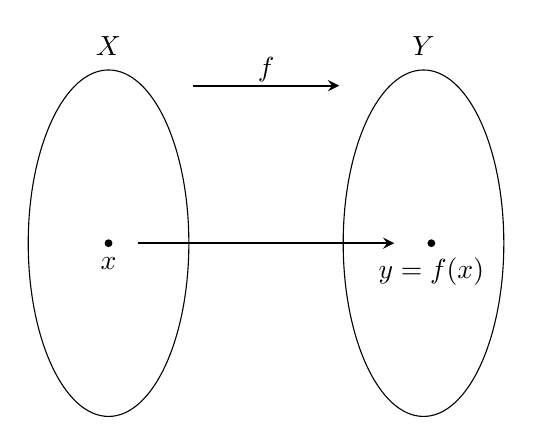
\begin{tikzpicture}[
		>=stealth,
		bullet/.style={
			fill=black,
			circle,
			minimum width=1pt,
			inner sep=1pt
		},
		projection/.style={
			->,
			thick,
			shorten <=2pt,
			shorten >=2pt
		},
		every fit/.style={
			ellipse,
			draw,
			inner sep=0pt
		}
		]
		\node at (2,4.7) {$f$};
		\draw[projection] (1,4.5) -- (3,4.5);
		\node at (0,5) {$X$};
		\node[bullet,label=below:$x$] at (0,2.5){};
		\node at (4,5) {$Y$};
		\node[bullet,label=below:{$y=f(x)$}] at (4.1,2.5){};
		\draw (0,2.5) ellipse (1.02cm and 2.2cm);
		\draw (4,2.5) ellipse (1.02cm and 2.2cm);
		\draw[projection] (0.3,2.5) -- (3.7,2.5);
		\end{tikzpicture}
	\end{center}
	
	\begin{definition}
		Two functions $ f $ and $ g $ are \textbf{equal} if they have the same domain and the same codomain and if $ f(x) = g(x) $ for all $ x $ in the domain.
	\end{definition}

	\begin{definition}
		The \textbf{graph} of $ f: X \to Y $ is the set
		\[ G_f = \{ (x,y) \in X \times Y | y= f(x) \} \]
	\end{definition}
	
	\subsubsection*{Some common functions}
	
	\begin{itemize}
		\item \textbf{Identity function} $ I_X: X \to X $ maps every element to itself,
			\[ \forall x \in X, \, i_X (x) = x \]
		\item \textbf{Polynomial function} of degree $ n $ with real coefficients $ a_0,a_1,\dots, a_n $ is a function from $ \R $ to $ \R $:
			\[ P_n(x) = a_0x^n + a_1 x^{n-1} + a_2 x^{n-2} + \dots + a_{n-1} x + a_n \]
			If $ a_0 \neq 0 $, then $ \deg P_n(x) = n $.
	\end{itemize}
	
	\subsection*{Range (or Image) of a Function}
	
	\begin{definition}
		Let $ f: X \to Y $ be a function. The \textbf{range} of $ f $ (also called the \textbf{image} of $ f $) is the set 
		\[ \{ y \in Y | y= f(x) \text{ for some } x \in X \} \]
	\end{definition}
	We denote the range (or image) of the function $ f $ by $ \ran f $ (or $ \image f $).
	
	\begin{center}
		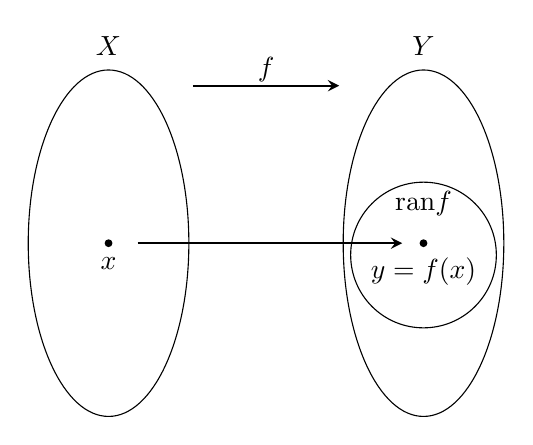
\begin{tikzpicture}[
		>=stealth,
		bullet/.style={
			fill=black,
			circle,
			minimum width=1pt,
			inner sep=1pt
		},
		projection/.style={
			->,
			thick,
			shorten <=2pt,
			shorten >=2pt
		},
		every fit/.style={
			ellipse,
			draw,
			inner sep=0pt
		}
		]
		\node at (2,4.7) {$f$};
		\draw[projection] (1,4.5) -- (3,4.5);
		\node at (0,5) {$X$};
		\node[bullet,label=below:$x$] at (0,2.5){};
		\node at (4,5) {$Y$};
		\node[bullet,label=below:{$y=f(x)$}] at (4,2.5){};
		\draw (0,2.5) ellipse (1.02cm and 2.2cm);
		\draw (4,2.5) ellipse (1.02cm and 2.2cm);
		\draw[projection] (0.3,2.5) -- (3.8,2.5);
		\draw (4,2.35) circle (9.25mm);
		\node at (4,3) {$\ran f$};
		\end{tikzpicture}
	\end{center}
	
	\begin{example}
		Let $ f: [\frac{1}{3}, \infty] \to \R $ be defined by $ f(x) = \sqrt{3x-1} $ and $ S = \{ y \in \R | y \geq 0 \} $. Prove that $ \ran f = S $.
	\end{example}

	\begin{proof}
		Let $ y \in \ran f $. Then $ y = f(x) $ for some $ x \in [\frac{1}{3}, \infty] $. But $ f(x) = \sqrt{3x-1} $, so $ y = \sqrt{3x-1} \geq 0 $ and hence $ y \in S $. Thus $ \ran f \subseteq S $.
		
		\noindent Conversely, let $ y \in S $. In order to show that $ y \in \ran f $, we must find $ x \in [\frac{1}{3}, \infty] $ such that $ f(x) = y $. Indeed, if $ x = \frac{y^2 + 1}{3} $ then $ x \in [\frac{1}{3}, \infty] $ (because $ y \in S \Rightarrow y \geq 0 \Rightarrow y^2 \geq 0 \Rightarrow y^2+1 \geq 1 \Rightarrow x = \frac{y^2+1}{3} \geq \frac{1}{3} $ ) and $ f(x) = f(\frac{y^2+1}{3}) = \sqrt{3\left( \frac{y^2+1}{3} \right) - 1} = \sqrt{y^2+1-1} = \sqrt{y^2} = |y| = y $ (since $ y \geq 0 $). Thus $ S \subseteq \ran f $.
	\end{proof}
	
	
	
	
	\section{Composition of Functions}
	
	\begin{definition}
		Let $ A,B,C $ be nonempty sets, and let $ f:A \to B $, $ g: B \to C $ be functions. we define a function
		\[ g \circ f: A \to C \]
		called the \textbf{composition} of $ f $ and $ g $, by
		\[ (g \circ f)(a) = g(f(a)) \]
	\end{definition}

	Using diagram,
	
	\begin{center}
		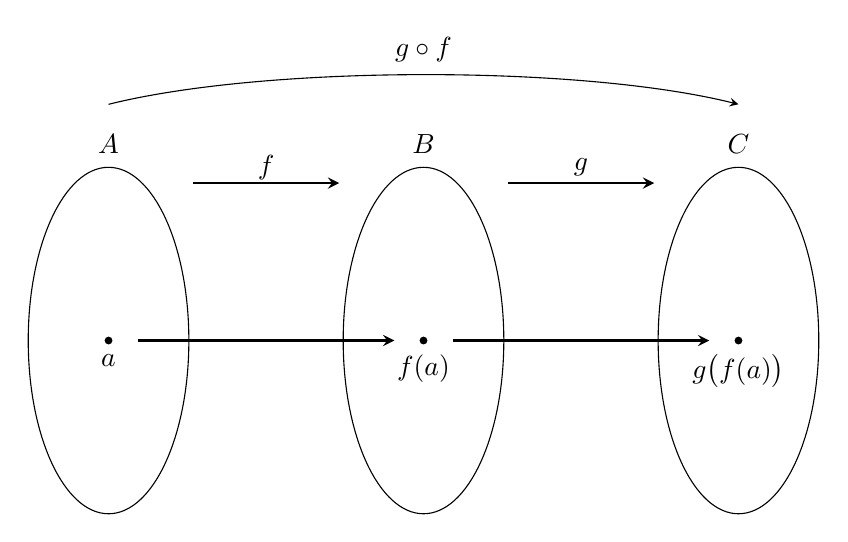
\begin{tikzpicture}[
		>=stealth,
		bullet/.style={
			fill=black,
			circle,
			minimum width=1pt,
			inner sep=1pt
		},
		projection/.style={
			->,
			thick,
			shorten <=2pt,
			shorten >=2pt
		},
		every fit/.style={
			ellipse,
			draw,
			inner sep=0pt
		}
		]
		\node at (2,4.7) {$f$};
		\draw[projection] (1,4.5) -- (3,4.5);
		\node at (0,5) {$A$};
		\node[bullet,label=below:$a$] (START)   at (0,2.5){};
		\node at (4,5) {$B$};
		\node[bullet,label=below:$f(a)$] at (4,2.5){};
		\node at (6,4.7) {$g$};
		\draw[projection] (5,4.5) -- (7,4.5);
		\node at (8,5) {$C$};
		\node[bullet,label=below:$g\big(f(a)\big)$] (END) at (8,2.5){};
		
		\draw [->] (0,5.5) .. controls (2,6) and (6,6) .. (8,5.5);
		\node at (4,6.2) {$g \circ f$};
		
		\draw (0,2.5) ellipse (1.02cm and 2.2cm);
		\draw (4,2.5) ellipse (1.02cm and 2.2cm);
		\draw (8,2.5) ellipse (1.02cm and 2.2cm);
		
		\draw[projection] (0.3,2.5) -- (3.7,2.5);
		\draw[projection] (4.3,2.5) -- (7.7,2.5);
		\end{tikzpicture}
		\newline
	\end{center}
	
	\begin{example}
		Let $ f,g: \R \to \R $ be defined by $ f(x) = e^x $ and $ g(x) = x \sin(x) $. Find $ f \circ g $ and $ g \circ f $.
	\end{example}	
	\noindent \textit{Solution.} First note that $ f \circ g: \R \to \R $ and $ g \circ f: \R \to \R $. Let $ x \in \R $.
	\begin{align*}
		&(f \circ g)(x) = f(g(x)) = f(x\sin(x)) = e^{x\sin(x)}\\
		&(g \circ f)(x) = g(f(x)) = g(e^x) = e^x \sin(e^x)
	\end{align*}
	We conclude that $ f \circ g \neq g \circ f $, so function composition is \textbf{not} commutative.
	
	\begin{proposition}
		Let $ f: A \to B $, $ g: B \to C $ and $ h: C \to D $. Then
		\[ (h \circ g) \circ f = h \circ (g \circ f) \]
	\end{proposition}
	
	\begin{proof}
		First note that $ (h \circ g) \circ f: A \to D $ and $ h \circ (g \circ f): A \to D $. Let $ x \in A $. Then $ ((h \circ g) \circ f)(x) = h(g(f(x))) $ and $ (h \circ (g \circ f))(x) = h(g(f(x))) $.
	\end{proof}
	
	h
	
	\section{Surjective and Injective Functions}
	
	
	
	
	
	
	
	
	
	
	
	
	
	
	
	
	
	
	
	
	
	
	
	
	
	\section{Invertible Functions}
	
	\section{Functions and Sets}
	
	
	\addcontentsline{toc}{chapter}{}
	\pagestyle{plain}

\end{document}
